\documentclass[12pt,a4paper]{article}
\usepackage[utf8]{inputenc}
\usepackage{amsmath}
\usepackage{amsfonts}
\usepackage{amssymb}
\usepackage[brazil]{babel}
\usepackage{indentfirst}
\usepackage{url}
\usepackage{listings}
\RequirePackage{graphicx}
\title{Relatório Chart.js}
\author{Adallberto Lucena Moura \and Andrey Silva Ribeiro \and Anny Karoliny Moraes Ribeiro \and Daniel Moreira Cardoso \and Davi Ildeu de Faria}
\usepackage[left=3cm,right=3cm,top=2cm,bottom=2cm]{geometry}

\usepackage{color}

\definecolor{mygreen}{rgb}{0,0.6,0}
\definecolor{mygray}{rgb}{0.5,0.5,0.5}
\definecolor{mymauve}{rgb}{0.58,0,0.82}

\lstset{ %
  backgroundcolor=\color{white},   % choose the background color; you must add \usepackage{color} or \usepackage{xcolor}; should come as last argument
  basicstyle=\footnotesize,        % the size of the fonts that are used for the code
  breakatwhitespace=false,         % sets if automatic breaks should only happen at whitespace
  breaklines=true,                 % sets automatic line breaking
  captionpos=b,                    % sets the caption-position to bottom
  commentstyle=\color{mygreen},    % comment style
  deletekeywords={...},            % if you want to delete keywords from the given language
  escapeinside={\%*}{*)},          % if you want to add LaTeX within your code
  extendedchars=true,              % lets you use non-ASCII characters; for 8-bits encodings only, does not work with UTF-8
  frame=single,	                   % adds a frame around the code
  keepspaces=true,                 % keeps spaces in text, useful for keeping indentation of code (possibly needs columns=flexible)
  keywordstyle=\color{blue},       % keyword style
  language=Octave,                 % the language of the code
  morekeywords={*,...},            % if you want to add more keywords to the set
  numbers=left,                    % where to put the line-numbers; possible values are (none, left, right)
  numbersep=5pt,                   % how far the line-numbers are from the code
  numberstyle=\tiny\color{mygray}, % the style that is used for the line-numbers
  rulecolor=\color{black},         % if not set, the frame-color may be changed on line-breaks within not-black text (e.g. comments (green here))
  showspaces=false,                % show spaces everywhere adding particular underscores; it overrides 'showstringspaces'
  showstringspaces=false,          % underline spaces within strings only
  showtabs=false,                  % show tabs within strings adding particular underscores
  stepnumber=2,                    % the step between two line-numbers. If it's 1, each line will be numbered
  stringstyle=\color{mymauve},     % string literal style
  tabsize=2,	                   % sets default tabsize to 2 spaces
  title=\lstname                   % show the filename of files included with \lstinputlisting; also try caption instead of title
}

\begin{document}
\begin{titlepage}


\begin{center}
\begin{figure}[htb]
		
		\label{figura:LogoIF}
	
		\centering
		
\includegraphics[width=6cm]{logo.png} 
\end{figure}


Instituto Federal Goiano - Campus Ceres\\
Bacharelado em Sistemas de Informação\\
Prof. Me. Ronneesley Moura Teles\\\vspace{0.2cm}
Adallberto Lucena Moura \\
Andrey Silva Ribeiro \\
Anny Karoliny Moraes Ribeiro \\
Daniel Moreira Cardoso \\
Davi Ildeu de Faria \\

\vspace{5.0cm}

\textit{\textbf{\Large{Relatório Chart.js}}}\\\vspace{0.5cm}
\vspace{9.5cm}

Outubro\\
2017\\
\end{center}
\end{titlepage}



\tableofcontents

\newpage
\begin{center}
\textbf{\Large{Relatório Chart.js}}\\\vspace{0.5cm}
\end{center}

\section{Introdução}

Chart.js é uma biblioteca desenvolvida por Nick Dowine sob a linguagem JavaScript, renderiza os gráficos utilizando o elemento canvas do HTML5. O Chart.js framework utiliza uma biblioteca para construção de maneira mais performática e fácil, ela é open source e disponível sob licença MIT no Github \url{https://github.com/chartjs/Chart.js}. Por ser open source, qualquer pessoa pode contribuir com a comunidade e manter sempre ativo, atualizado com novas features.

O Chart.js possui 8 tipos diferentes de gráficos, entre os tradicionais como barra e pizza. Há um suporte responsivo, possui legenda para os gráficos e opções de gráficos interativos e modulares.


\section{Tipos de gráficos}
Alguns exemplos de gráficos que podem ser gerados:
\begin{figure}[!htb]
\centering
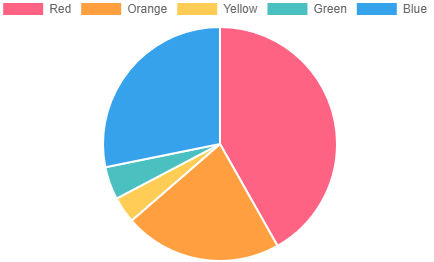
\includegraphics[width=18cm]{recursos/PieChart.png}
\label{Pie}
\caption{Pie Chart / Gráfico de Torta. Fonte: http://www.chartjs.org/samples/latest/charts/pie.html; Acesso em 20/10/2017.}
\end{figure}

\begin{figure}[!h]
\centering
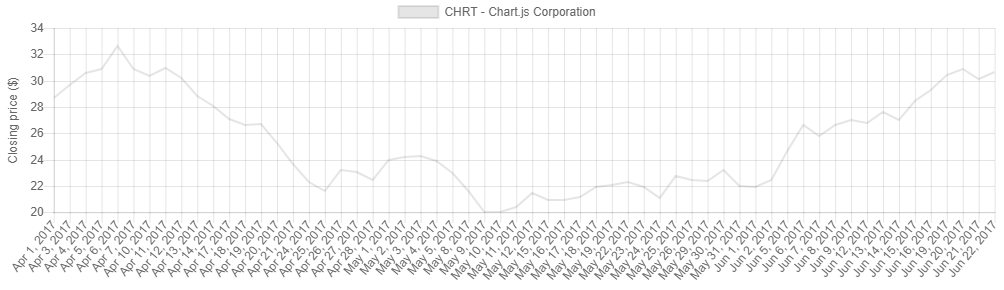
\includegraphics[width=13cm]{recursos/LineChart.png}
\label{Line}
\caption{Line Chart / Gráfico de linha. Fonte: http://www.chartjs.org/samples/latest/scales/time/financial.html; Acesso em 20/10/2017.}
\end{figure}

\begin{figure}[!h]
\centering
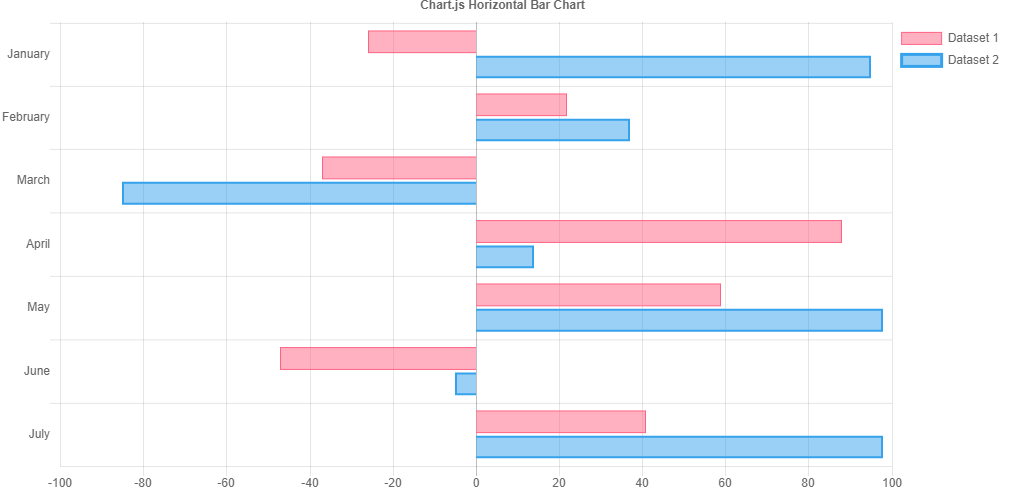
\includegraphics[width=13cm]{recursos/BarChart.png}
\label{Bar}
\caption{Horizontal Bar Chart / Gráfico de barra horizontal. Fonte: http://www.chartjs.org/samples/latest/charts/bar/horizontal.html; Acesso em 20/10/2017.}
\end{figure}

\begin{figure}[!h]
\centering
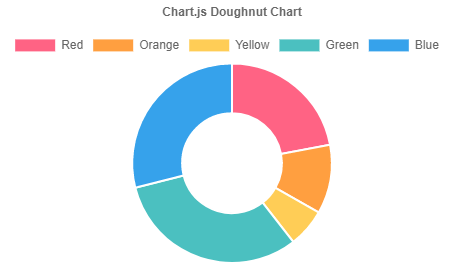
\includegraphics[width=13cm]{recursos/DoughnutChart.png}
\label{Doughnut}
\caption{Doughnut Chart / Gráfico de Rosquinha. Fonte: http://www.chartjs.org/samples/latest/charts/doughnut.html; Acesso em 20/10/2017.}
\end{figure}


\begin{figure}[!h]
\centering
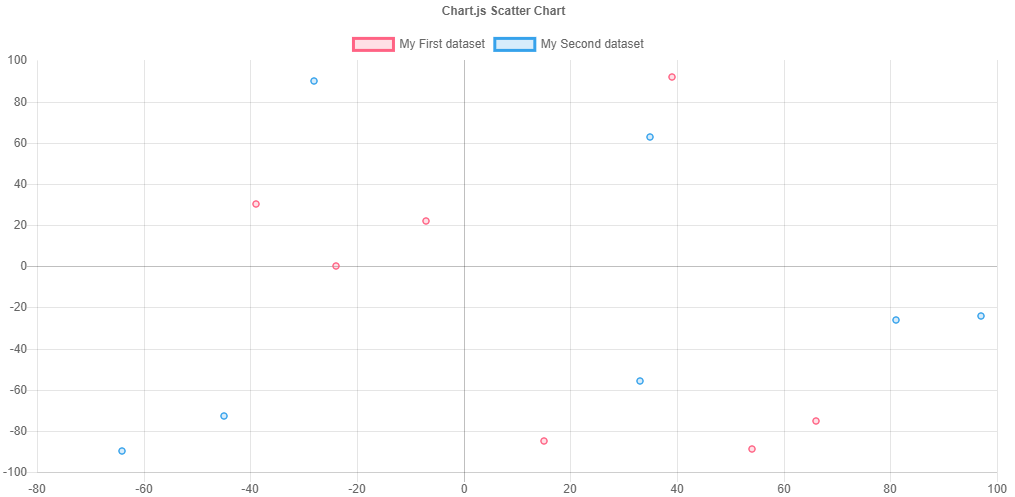
\includegraphics[width=11cm]{recursos/ScatterChart.png}
\label{Scatter}
\caption{Scatter Chart / Gráfico de Dispersão. Fonte: http://www.chartjs.org/samples/latest/charts/scatter/basic.html; Acesso em 20/10/2017.}
\end{figure}


\section{Exemplos de gráficos implementados.}

\subsection{Gráfico de linhas} 
\lstinputlisting{recursos/linhas.html}

\subsection{Gráfico Polar}
\lstinputlisting{recursos/polar.html}

\subsection{Gráfico Radar}
\lstinputlisting{recursos/radar.html}

\section{Vantagens}
\begin{itemize}
\item O código é open source e está disponível na página do Github;
\item Tem continuidade;
\item Tem compatibilidade com outros tipos de navegadores;
\item A biblioteca possui uma documentação oficial dentro da página do projeto;
\item Existe uma comunidade ativa no Github;
\item Possui exemplos de código na página do projeto.
\end{itemize}

\section{Conclusão}
Para aqueles que desejam adicionar gráficos na web, sendo para pequenos projetos ou em um dashboard de uma página de adm back end, por exemplo, o Chart.js é uma perfeita escolha, já que os gráficos são todos responsivos e personalizáveis, podendo assim se adaptar a qualquer tamanho de tela, ter suas cores mudadas entre outras coisas que são todas passiveis de personalização. 
	
Outro ponto bastante interessante é que o Chart.js e extremamente leve se comparado com outras bibliotecas e não possui dependências. 

Também podemos combinar o código da biblioteca com PHP, Java e outras linguagens, para incluir os dados a partir de um banco de dados e automatizar a atualização dos gráficos.

\end{document}